%This is the first chapter of the dissertation

%The following command starts your chapter. If you want different titles used in your ToC and at the top of the page throughout the chapter, you can specify those values here. Since Columbia doesn't want extra information in the headers and footers, the "Top of Page Title" value won't actually appear.

\chapter[Event Reconstruction][Top of Page Title]{Event Reconstruction}

This chapter describes the reconstruction algorithms used within ATLAS.\todo{cite fermilab lectures}
We will make the distinction between the ``primitive'' objects which are reconstructed from the detector signals from the ``composite'' physics objects we use in measurements and searches for new physics.

\section{Primitive Object Reconstruction}

The primitive objects reconstructed by ATLAS are \textit{tracks} and (calorimeter) \textit{topoclusters}.
These are reconstructed directly from tracking hits and calorimeter energy deposits into cells.
Tracks can be further divided into inner detector and muon spectrometer tracks.

\subsection{Inner Detector Tracks}
\todo{cite paper/note}

\subsection{Calorimeter Topoclusters}
\todo{cite paper/note}

Topoclusters are the output of the algorithm used within ATLAS to combine calorimeter cells in a way which extracts signal from a background of significant electronic noise\cite{PERF-2014-07}.
They are the primary input to the algorithms which reconstruct jets, photons, and electrons.

Topological clusters are reconstructed from calorimeter cells in the following way.
First, one maps all (hadronic or electromagnetic) cells onto a single $\eta-\phi$ plane so one can speak of \textit{neighboring} cells.
Two cells are considered neighboring if they are in the same layer and directly adjacent, or if they are in adjacent layers and overlap in $\eta-\phi$ space.
The \textit{significance} $\xi_{\text{cell}}$ of a cell during a given event is

\begin{equation}
\calosig = \frac{E_{\text{cell}}}{\sigma_{\text{noise,cell}}}
\end{equation}

where $\sigma_{\text{noise,cell}}$ is measured for each cell in ATLAS and $E_{\text{cell}}$ measures the current energy level of the cell.
One thiks of this as the measurement of the energy \textit{over threshold} for the cell.

Topocluster \textit{seeds} are defined as calorimeter cells which have a significance $\calosig > 4 $.
These are the inputs to the algorithm; one iteratively tests all cells adjacent to these seeds for $\calosig > 2$.
Each cells passing this selection is then added to the topocluster, and the procedure is repeated.
When the algorithm reaches the point where there are no additional adjacent cells with $\calosig > 2$, every positive-energy cell adjacent to the current proto-cluster is added.
This collection of cells is summed; the summed object is known as a topocluster.
An example of this procedure for a simulation dijet event is shown in Fig.\ref{fig:topocluster}.
\begin{figure}
\caption{Example of topoclustering on a simulated dijet event.} \label{fig:topocluster}
\subfloat[All cells with $\calosig > 4$.]{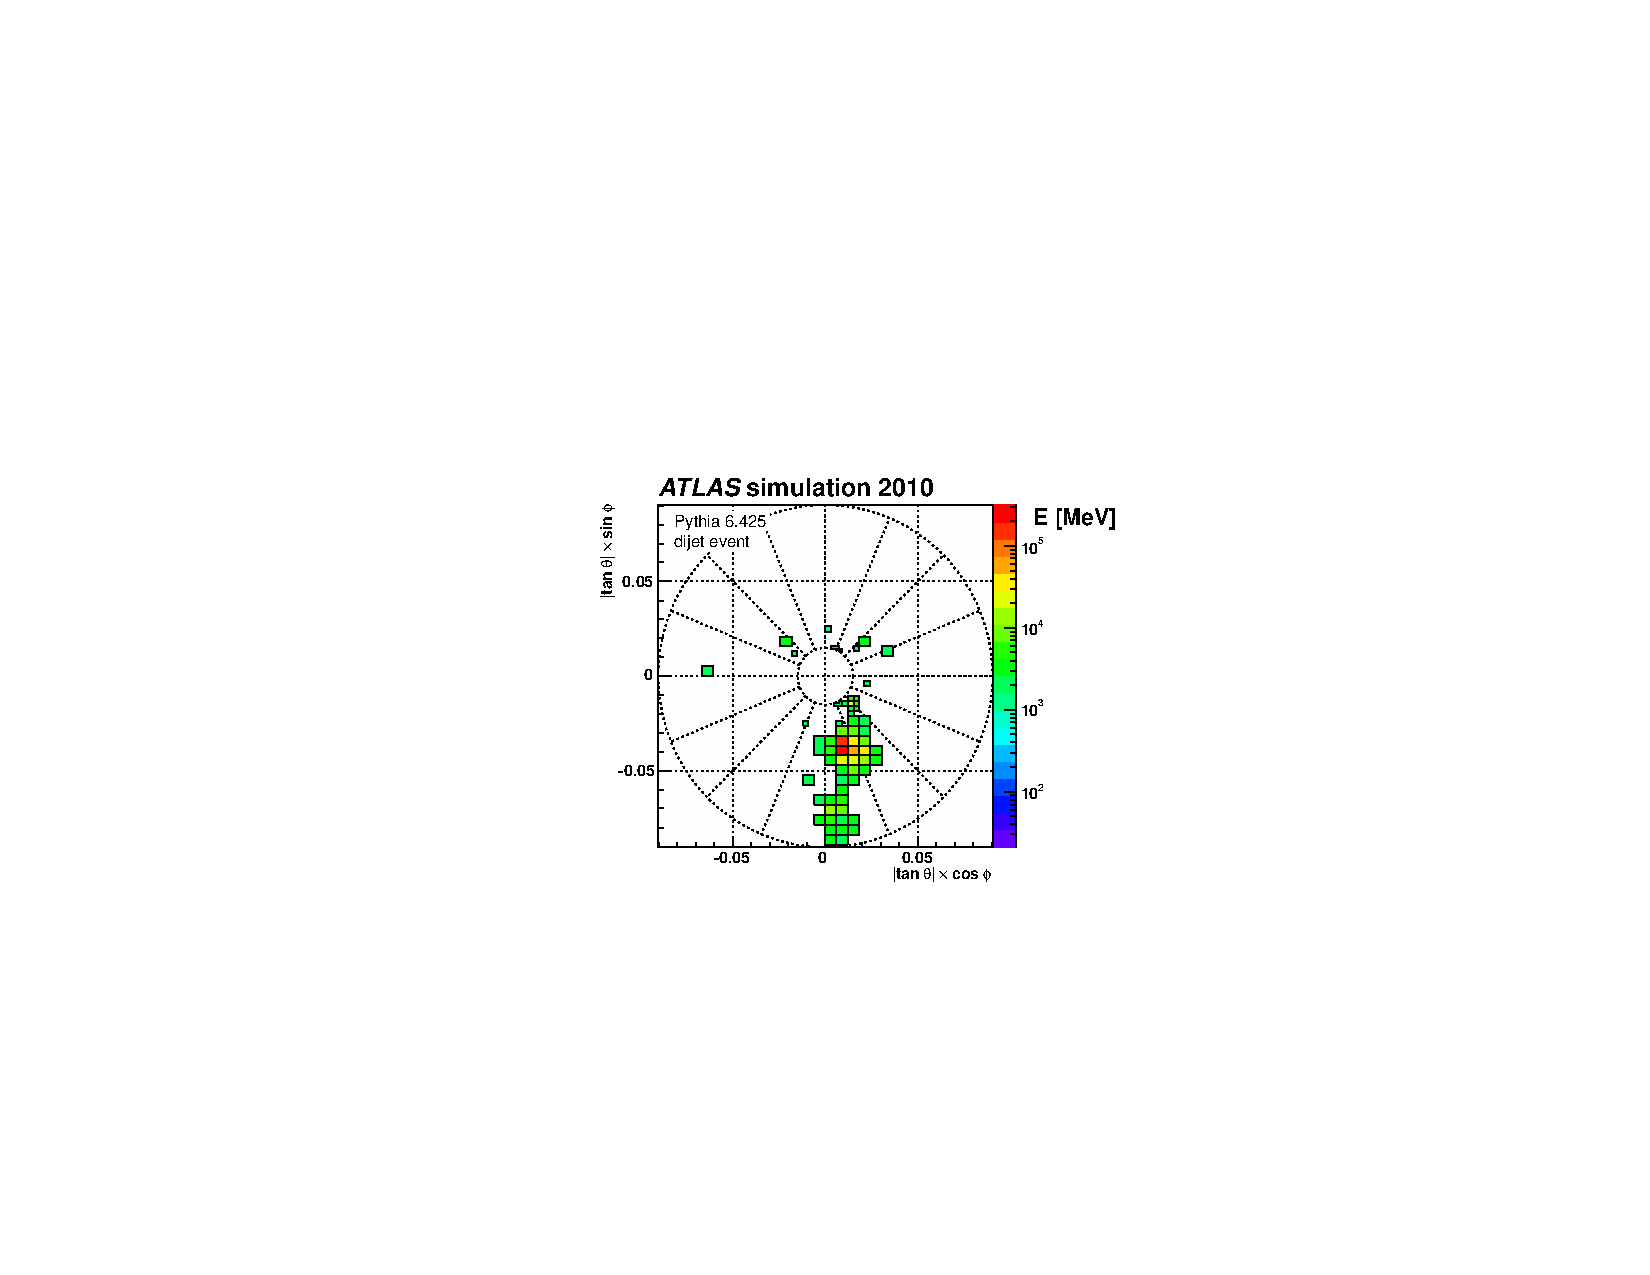
\includegraphics[width=.45\linewidth]{topoclustering_sig4.pdf}}
\subfloat[All cells with $\calosig > 2$.]{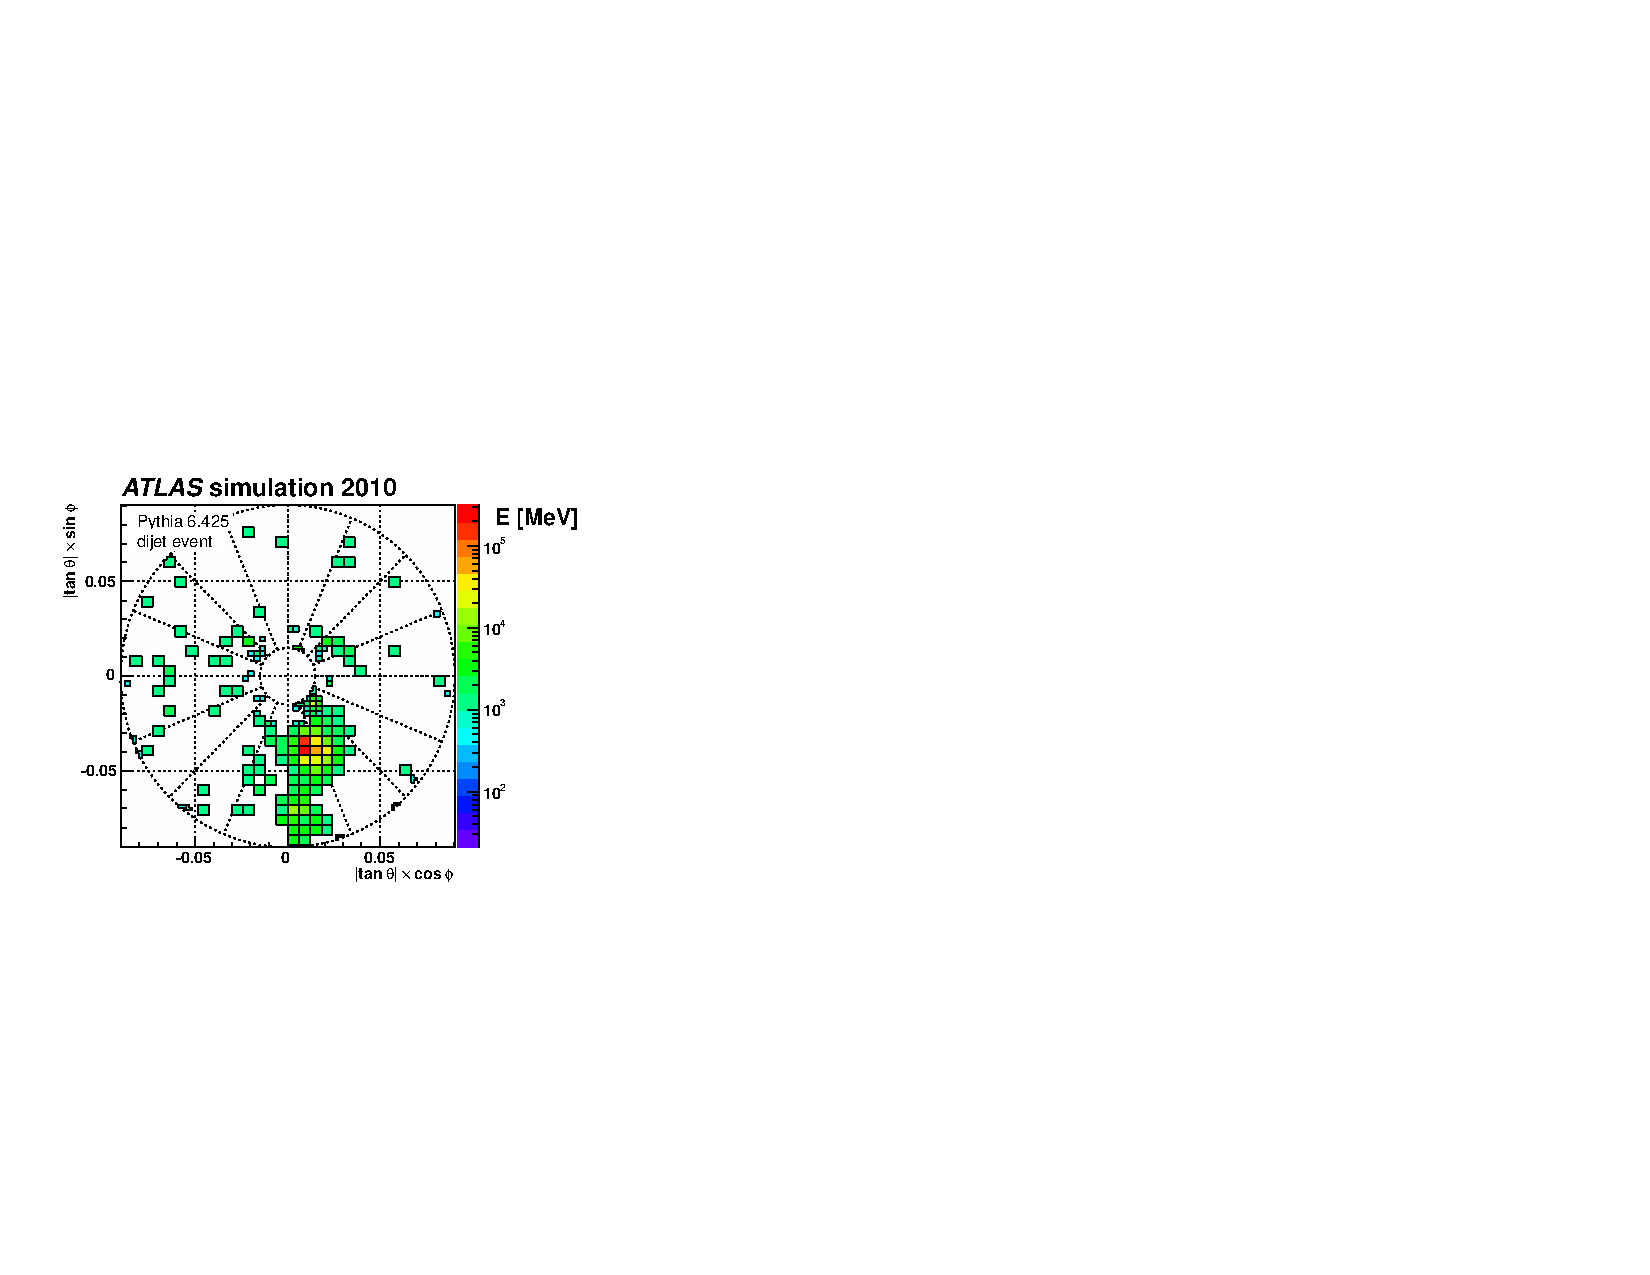
\includegraphics[width=.45\linewidth]{topoclustering_sig2.pdf}} \\
\subfloat[All clustered cells.]{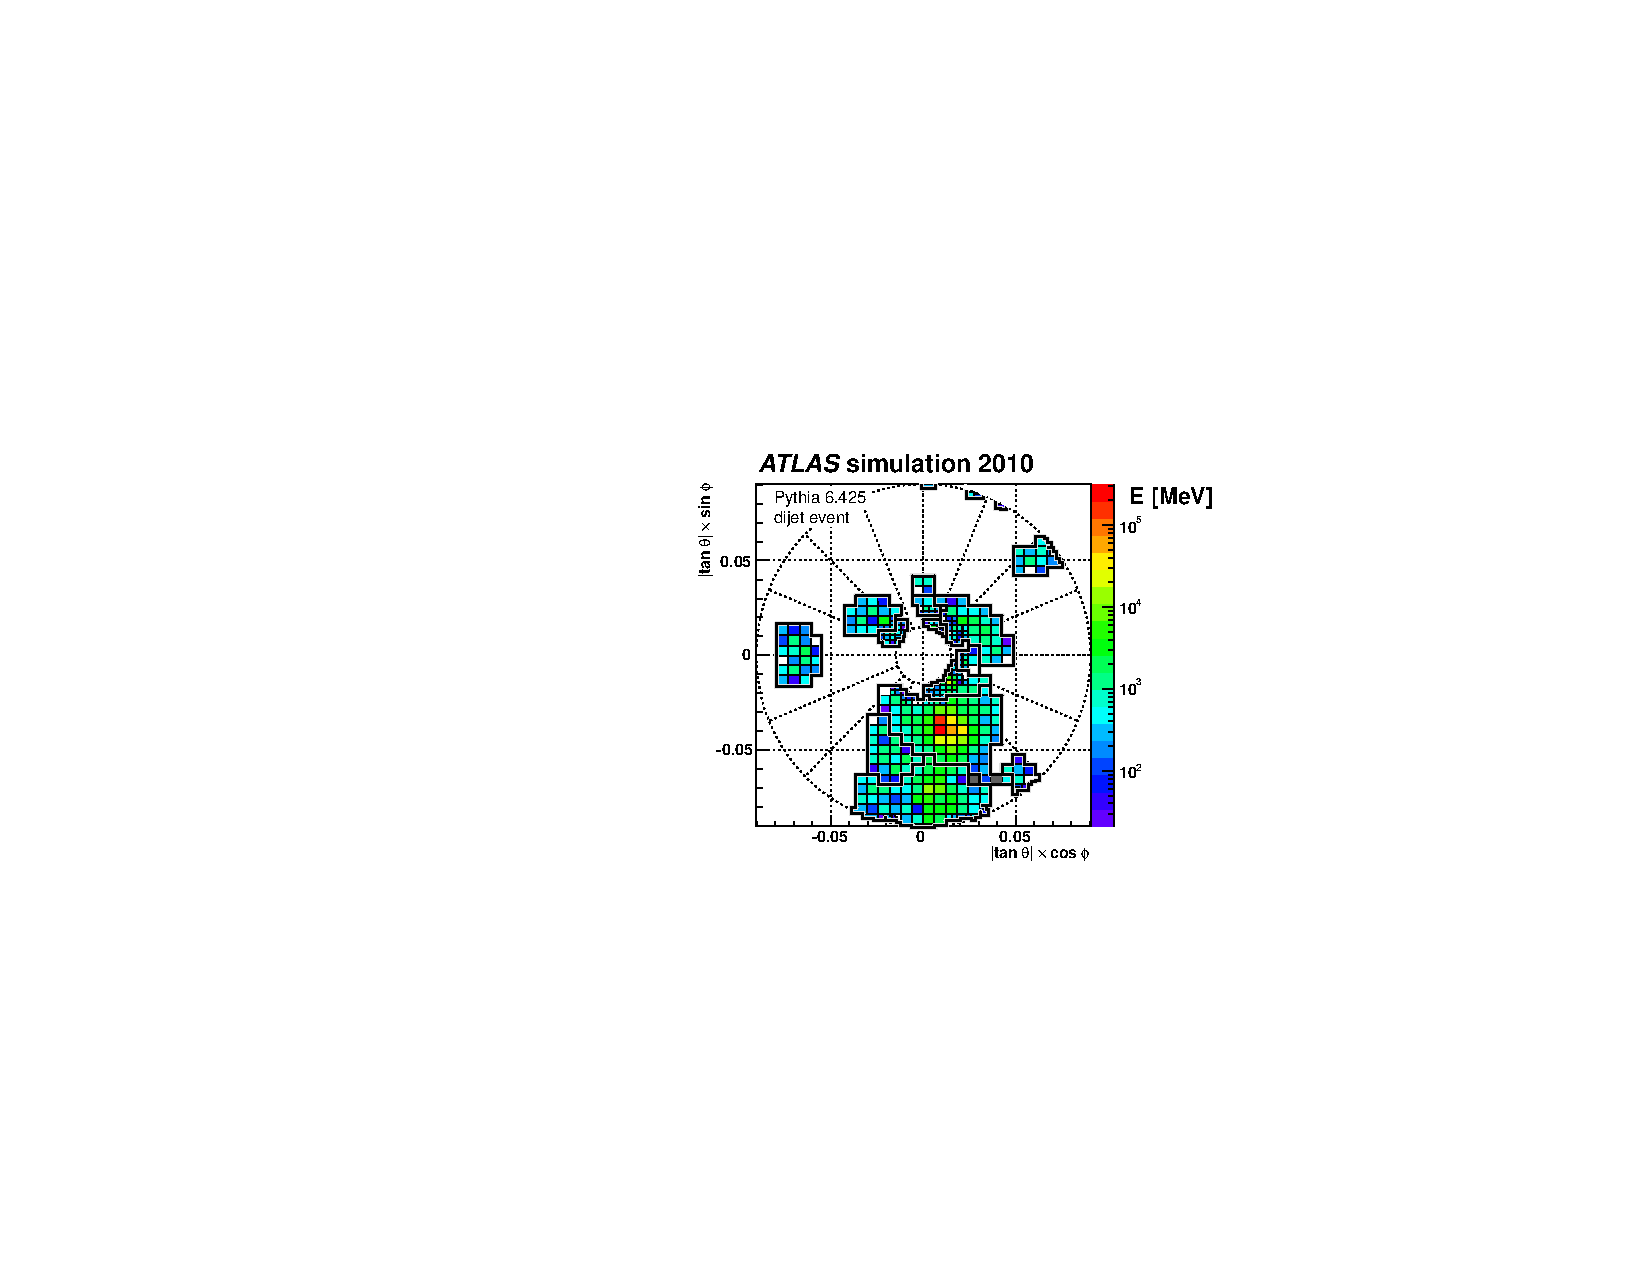
\includegraphics[width=.9\linewidth]{topoclustering_sig0.pdf}}
\end{figure}

\subsection{Muon Spectrometer Tracks}

\section{Physics Object Reconstruction}

There are essentially five objects used in ATLAS searches for new physics: electrons, photons, muons, jets, and \met.
The reconstruction of these objects is described here.
A very convenient summary plot is shown in Fig.\ref{
In this thesis, we present a search for new physics in a zero lepton final state; we will provide additional details about jet and \met reconstruction.
% \subsection{Vertices}

% Vertex reconstruction is an important first step in the reconstruction of ATLAS events\cite{ATL-INDET-PUB-2009-001}.
% If two tracks from charged particles point at the same place inside the detector, we can associate these tracks to that point, which we then call a vertex.
% Generally, we speak of primary vertices associated
% \begin{figure}
% \caption{Depiction of different vertices reconstruct by ATLAS.
% Each ATLAS event has the primary vertex, b-physics vertices, and pileup vertices.} \label{fig:topocluster}
% 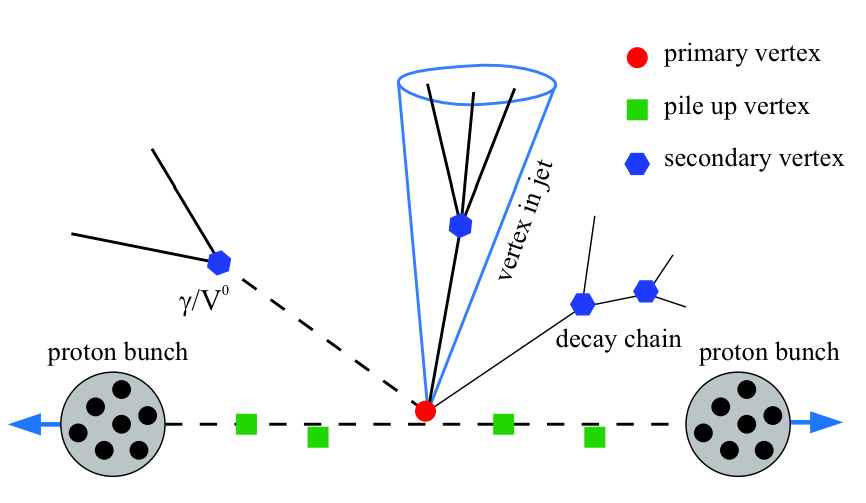
\includegraphics[width=.45\linewdith]{vertex_reconstruction} \\
% \end{figure}

\subsection{Electrons}

Electrons are identified \cite{PERF-2013-03}
\todo{cite paper/note}

\subsection{Photons}
\todo{cite paper/note}

\subsection{Muons}
\todo{cite paper/note}

\subsection{Jets}
\todo{cite paper/note}

\subsection{Missing Transverse Momentum}
\todo{cite paper/notes}

\section{Maybe PFlow?}